\documentclass{article}
\usepackage{graphicx}
\begin{document}
In the implementation of Preflow algrithms, we differentiate
two types of \textbf{push}. One is normal push, that is,
$f_{uv} < c_{uv}$ and $x_u >0$, $u$ can push some stored flow
to $v$. The other is \textbf{push back}, that is,
$f_{vu} >0$ and $x_u >0$ and $u$ can push some stored flow back to $v$.

\begin{figure}[!ht]
\centering
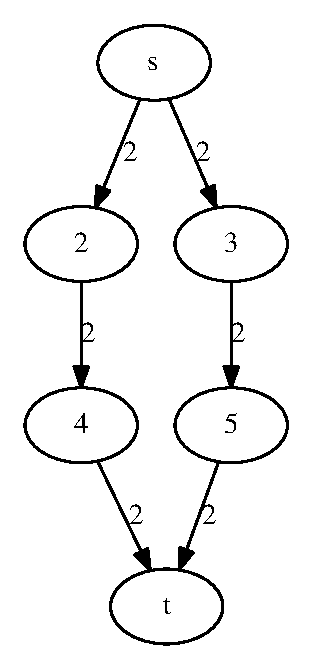
\includegraphics[width=6cm]{fig/size.eps}
\caption{minimum cut is not unique}\label{fig:mc}
\end{figure}

In figure \ref{fig:mc}, our algrithm (Preflow_Relabel) will produce the minimum cut whose source side is of maximal size.

\begin{figure}[!ht]
\centering
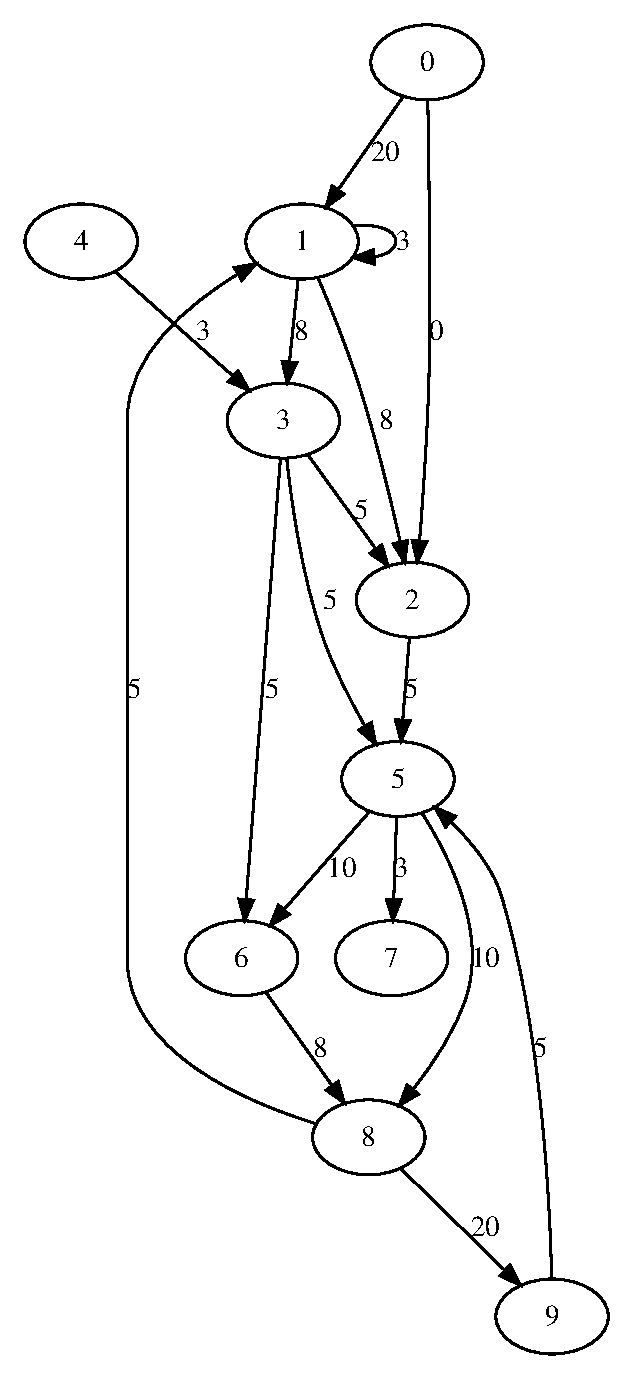
\includegraphics[width=6cm]{fig/test.eps}
\caption{minimum cut is not unique}\label{fig:ex}
\end{figure}

Figure \ref{fig:ex} is the official example of lemon library when testing Preflow algorithm, notice that Node 0 and Node 7 will never be reached. Therefore, their belonging in min-cut seems arbitrary. 
\end{document}
